\begin{figure}[H]
	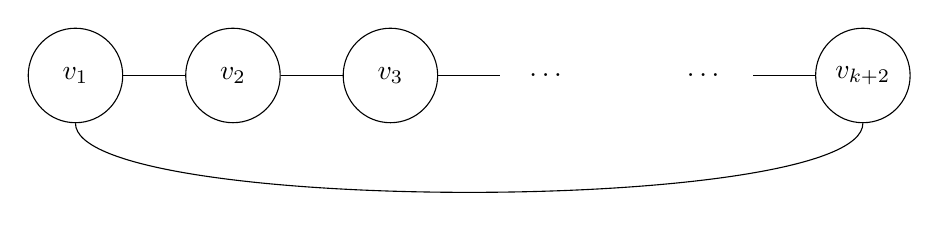
\begin{tikzpicture}[node distance={20mm}, main/.style = {draw, circle}, minimum size=1.2cm]
		\node[main] (1) {$v_1$};
		\node[main] (2) [right of=1] {$v_2$};
		\node[main] (3) [right of=2] {$v_3$};
		\node (4) [right of =3] {\dots};
		\node (5) [right of =4] {\dots};
		\node[main] (6) [right of=5] {$v_{k + 2}$};
		\draw (1) -- (2);
		\draw (2) -- (3);
		\draw (3) -- (4);
		\draw (5) -- (6);
		\draw (6) to [out=-90,in=-90,looseness=0.3] (1);
	\end{tikzpicture}
	\centering
	\caption{Structure $\mathfrak{A}$, consisting of a cycle of length $k + 2$.}
\end{figure}